\documentclass[11pt]{article}

% -- Color scheme

% Color package
\usepackage{xcolor}
\usepackage{varwidth}
\usepackage{parskip}
% Color scheme definitions

% Default
\definecolor{minimal-main}{HTML}{131313}
\definecolor{minimal-light}{HTML}{F2F2F2}
\definecolor{minimal-contrast}{HTML}{F3F2F5}

% Blue
%\definecolor{minimal-main}{HTML}{1E2839}
%\definecolor{minimal-light}{HTML}{EFF4F9}
%\definecolor{minimal-contrast}{HTML}{F3F2F5}

% Green
%\definecolor{minimal-main}{HTML}{083031}
%\definecolor{minimal-light}{HTML}{DEECE9}
%\definecolor{minimal-contrast}{HTML}{F3F2F5}

% Red
%\definecolor{minimal-main}{HTML}{361222}
%\definecolor{minimal-light}{HTML}{FFE8F2}
%\definecolor{minimal-contrast}{HTML}{F3F2F5}

% Additional color definitions
\definecolor{minimal-black}{HTML}{131313}
\definecolor{minimal-white}{HTML}{F3F2F5}
\definecolor{minimal-red}{HTML}{C43C2D}
\definecolor{minimal-blue}{HTML}{343454}
\definecolor{minimal-yellow}{HTML}{F1C40F}
\definecolor{minimal-green}{HTML}{2D6514}
\definecolor{minimal-beige}{HTML}{D7B6A5}

% Colorbox environments
\usepackage[most]{tcolorbox}


% -- Page layout

% Layout adjustments of page (a4 without margin)
\usepackage[paperheight=842pt, paperwidth=595pt, margin=0pt]{geometry}

% Remove paragraph indentation
\setlength{\parindent}{0pt}

% Interline spacing options
\newcommand{\largespace}{\\[2pt]}
\newcommand{\mediumspace}{\\[-3pt]}
\newcommand{\smallspace}{\\[-5pt]}

% In-box spacing around content
\newcommand{\inboxspacing}{.015\paperheight}

% Horizontal spacing of the boxes (must sum up to 1)
\newcommand{\sideboxwidth}{.35}
\newcommand{\mainboxwidth}{.65}

% Vertical spacing of the boxes (must sum up to 1)
\newcommand{\headboxheight}{.080}
\newcommand{\mainboxheight}{.910}
\newcommand{\footboxheight}{.010}

%   sideboxwidth           mainboxwidth
%  <------------> <---------------------------->
%  _____________________________________________
% |#############################################| ^
% |#############################################| |
% |################## HEADBOX ##################| | headboxheight
% |#############################################| |
% |#############################################| v
% |///////////////                              | ^
% |///////////////                              | |
% |///////////////                              | |
% |///////////////                              | |
% |////   ////////                              | |
% |//// S ////////              M               | |
% |//// I ////////              A               | |
% |//// D ////////              I               | |
% |//// E ////////              N               | | mainboxheight
% |//// B ////////              B               | |
% |//// O ////////              O               | |
% |//// X ////////              X               | |
% |////   ////////                              | |
% |///////////////                              | |
% |///////////////                              | |
% |///////////////                              | |
% |///////////////                              | v
% |#############################################| ^
% |################## FOOTBOX ##################| | footboxheight
% |#############################################| v


% -- Font settings

% Typesetting packages
\usepackage[letterspace=20]{microtype}
\usepackage[T1]{fontenc}

% Raleway font family
\usepackage[semibold]{raleway}
\renewcommand{\familydefault}{\sfdefault}

% Custom font commands
\newcommand{\header}[3]{\uppercase{\textbf{\fontsize{30}{100}{\lsstyle{#1 \hspace{3pt} #2 \hspace{3pt} #3}}}}}
\newcommand{\titlefont}[1]{\uppercase{\textbf{\Large{#1}}}}


% -- Additional packages

% Multirow tables
\usepackage{multirow}

% Settings for entire table columns (e.g \begin{tabular}{>{\footnotesize}rl})
\usepackage{array}

% Tikzpicture graphics
\usepackage{tikz}

% Clickable URLs
\usepackage{hyperref}
\urlstyle{same}


\begin{document}

\begin{tcbposter}[
    poster = {columns=1, rows=1, spacing=0pt},
    boxes = {sharp corners, halign=center, valign=center, boxrule=0pt}
]


% -- Headbox

\posterbox[
    colback=minimal-main,
    halign=center]
    {name=headbox,
    span=1,
    rowspan=\headboxheight}
{

    \color{white}

    \header{Lombardi}{Juan}{Manuel}

    \vspace{-7px}
    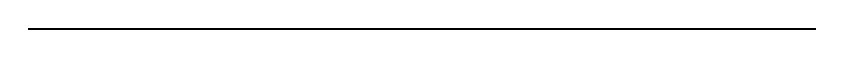
\begin{tikzpicture}
        \draw[fill=white] (-5.0, -0.01) rectangle (5.0, 0.01);
    \end{tikzpicture}
    \vspace{5px}

    \titlefont{PhD student}
}


% -- Sidebox

\posterbox[
    colback=minimal-light,
    valign=top,
    top=\inboxspacing,
    halign=right,
    right=\inboxspacing]
    {name=sidebar,
    below=headbox,
    column=1,
    span=\sideboxwidth,
    rowspan=\mainboxheight}
{

    \begin{tabular}{rl}

    \multicolumn{2}{@{}c@{}}{\includegraphics[width=1.0\textwidth]{images/Foto.png}} \\
    \mediumspace

        & \titlefont{Contact} \\
        \hline \mediumspace

        \multirow{4}{*}{\scalebox{0.075}{\input{icons/address.tex}}}
            & \textbf{Address} \\
                & Rosario \\
                & Argentina \\
                & \smallspace

        \multirow{2}{*}{\scalebox{0.075}{\input{icons/phone.tex}}}
            & \textbf{Phone} \\
                & \href{tel:+5493416492630}{+54 9 3416 49-2630} \\
                & \smallspace

        \multirow{2}{*}{\scalebox{0.075}{\input{icons/email.tex}}}
            & \textbf{E-Mail} \\
                & \href{mailto:jmlombardi@live.com}{jmlombardi@live.com} \\
                & \largespace

        & \titlefont{Personal} \\
        \hline \mediumspace

        \multirow{2}{*}{\scalebox{0.075}{\input{icons/birthday.tex}}}
            & \textbf{Date of Birth} \\
                & 31/12/1993 \\
                & \smallspace

        \multirow{2}{*}{\scalebox{0.075}{\input{icons/nationality.tex}}}
            & \textbf{Nationality} \\
                & Argentine \\
                & \largespace

        & \titlefont{Platforms} \\
        \hline \mediumspace

        \multirow{2}{*}{\scalebox{0.075}{\input{icons/github.tex}}}
            & \textbf{GitHub} \\
                & \href{https://github.com/AkarisDimitry}{Link} \\
                & \smallspace

        %\multirow{2}{*}{\scalebox{0.075}{\input{icons/linkedin.tex}}}
        %    & \textbf{LinkedIn} \\
        %        & \href{https://youtu.be/dQw4w9WgXcQ}{Carl Friedrich Gauss} \\
        %        & \largespace

        & \titlefont{Languages} \\
        \hline \mediumspace

        \multirow{2}{*}{\scalebox{0.075}{
\begin{tikzpicture}

\definecolor{red}{RGB}{179,25,66}
\definecolor{yellow}{RGB}{220,220,0}

    % Clip mask
    \clip (0, 3) circle (7);

  % Draw the red stripes
  \fill[minimal-red] (-9,6) rectangle (9,10);
  \fill[minimal-red] (-9,-4) rectangle (9,0);

  % Draw the yellow stripe
  \fill[minimal-yellow] (-9,0) rectangle (9,6);

\end{tikzpicture}}}
            & \textbf{Espanish} \\
                & Native \\
                & \smallspace

        \multirow{2}{*}{\scalebox{0.075}{
\definecolor{red}{RGB}{179,25,66}
\definecolor{white}{RGB}{255,255,255}
\definecolor{blue}{RGB}{10,48,78}


\begin{tikzpicture}

    % Clip mask
    \clip (0, 7) circle (7);
    
  % Draw the red stripes
  \foreach \i in {0,2,...,12}
    \fill[red] (-9,\i) rectangle (9,{\i+1});

  % Draw the white stripes
  \foreach \i in {1,3,...,13}
    \fill[white] (-9,\i) rectangle (9,{\i+1});

  % Draw the blue field
  \fill[blue] (-9,7) rectangle (-1,14);

  % Draw the stars: 5 rows of 6 stars
  \foreach \i in {-8,-6,...,-2}
    \foreach \j in {8,9,...,12}
      \node at (\i,\j) {\textcolor{white}{\Large{$\star$}}};

  % Draw the stars: 4 rows of 5 stars
  \foreach \i in {-7,-5,...,-3}
    \foreach \j in {8.5,9.5,...,11.5}
      \node at (\i,\j) {\textcolor{white}{\Large{$\star$}}};



\end{tikzpicture}}}
            & \textbf{English} \\
                & Fluent \\
                & \smallspace

        \multirow{2}{*}{\scalebox{0.075}{\input{flags/france.tex}}}
            & \textbf{French} \\
                & Basic \\
                & \smallspace
                
        \multirow{2}{*}{\scalebox{0.075}{\input{flags/germany.tex}}}
            & \textbf{German} \\
                & Basic (learning)

    \end{tabular}
}


% -- Mainbox

\posterbox[
    colback=white,
    valign=top,
    top=\inboxspacing,
    halign=left,
    left=\inboxspacing]
    {name=mainbox,
    column*=1,
    span=\mainboxwidth,
    below=headbox,
    rowspan=\mainboxheight}
{

    \begin{tabular}{>{\footnotesize}rl}

        & \titlefont{Education} \\
        \hline \mediumspace

        02/2013 - 10/2017
            & \textbf{Universidad Nacional de Rosario} \\
            & \href{https://www.fbioyf.unr.edu.ar/?page_id=594}{Degree in Chemistry} \\
            & \href{https://www.fbioyf.unr.edu.ar/}{Facultad De Ciencias Bioquímicas} \\& \href{https://www.fbioyf.unr.edu.ar/}{Y Farmacéuticas} \\
            & \smallspace

        04/2018 - Ongoing  
        & \textbf{Universidad Nacional de Rosario} \\
            expected completion   & Phd. in Physics \\
          date: 09/2023   &  \href{https://web.fceia.unr.edu.ar/es/}{Facultad de Ciencias Exactas, ingeniería} \\ & \href{https://web.fceia.unr.edu.ar/es/}{y agrimensura} \\
            & Topic: Theoretical study of electronic properties  \\& and reactivity of SAMs, MONCs and organic \\& molecules on metal surfaces.  \\
            & \href{https://bit.ly/3OrhjK1}{Supervisor: Dr. Paula Natalia Abufager}\\
            & \href{https://bit.ly/43sSVMb}{Co-Supervisor: Dr. Heriberto Fabio Busnengo} \\
            & \smallspace
            & \largespace

            %\href{https://www.conicet.gov.ar/new_scp/detalle.php?keywords=&id=24274&datos_academicos=yes}{Dr. Paula Natalia Abufager} 
            % \\
            
        & \titlefont{Publications} \\
        \hline \mediumspace



        2023
            & \textbf{Structure and stability of metallo-porphyrin} \\ & \textbf{networks on Au(111)} \\
            & J. M. Lombardi, D. Grumelli, R. Gutzler, \\ & H. F. Busnengo y P. Abufager. \\
            & \href{https://doi.org/10.1021/acs.jpcc.3c00579}{J. Phys. Chem. C 2023, 127, 13, 6569–6577} \\
            & \smallspace


        2020
            & \textbf{Enhancing Hydrogen Evolution Activity of Au(111)} \\ & \textbf{in Alkaline Media Through Molecular Engineering} \\ & \textbf{of a 2D Polymer} \\
            & P. Alexa, J. M. Lombardi, P. Abufager, \\ & H. F. Busnengo, D. Grumelli, V. S. Vyas, F. Haase, \\ & B Lotsch,R. Gutzer, K. Kern \\
            & \href{https://doi.org/10.1002/anie.201915855}{Angewandte Chemie 59 8411-8415}  \\
            & \smallspace

        2020
            & \textbf{Three-way calibration using PARAFAC and} \\ 
            & \textbf{MCR-ALS with previous synchronization of} \\ 
            & \textbf{second-order chromatographic data through a}  \\ 
            & \textbf{new functional alignment of pure vectors for the}  \\ 
            & \textbf{quantification in the presence of retention}  \\ 
            & \textbf{time shifts in peak position and shape} \\
            & S.Mazivila, J.M.Lombardi,  R.Páscoa, S.Bortolato, \\ 
            & J.Leitão, J.Silva\\
            & \href{https://doi.org/10.1016/j.aca.2020.12.033}{Analytica Chimica Acta. 1146. 98-108}  \\
            & \smallspace
            
        2018
            & \textbf{Functional data analysis, a new approach to} \\ & \textbf{aligning three-way liquid chromatographic} \\ & \textbf{with fluorescence detection data.} \\
            & J.M.Lombardia, S.A.Bortolato, \\ & \href{https://doi.org/10.1016/j.microc.2018.06.041}{Microchemical Journal 142, 219-228} \\          
            & \smallspace
            

    \end{tabular}
}

% -- Footbox
\posterbox[colback=minimal-main]
           {name=blankbox2,
           below=sidebar,
           column=1,
           span=1,
           rowspan=\footboxheight}{}

\posterbox[colback=minimal-main]
           {name=blankbox2,
           below=sidebar,
           column=1,
           span=1,
           rowspan=\footboxheight}{}

\end{tcbposter}

\newpage





\begin{tcbposter}[
    poster = {columns=1, rows=1, spacing=0pt},
    boxes = {sharp corners, halign=center, valign=center, boxrule=0pt}
]

% -- Headbox
\posterbox[
    colback=minimal-main,
    halign=center]
    {name=headbox,
    span=1,
    rowspan=\headboxheight}
{
    \color{white}

    \header{Lombardi}{Juan}{Manuel}

    \vspace{-7px}
    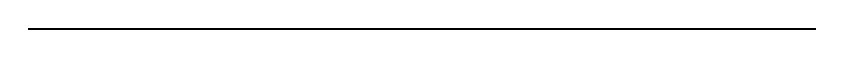
\begin{tikzpicture}
        \draw[fill=white] (-5.0, -0.01) rectangle (5.0, 0.01);
    \end{tikzpicture}
    \vspace{5px}

    \titlefont{PhD student}
}




% -- Mainbox de la segunda página

\posterbox[
    colback=white,
    valign=top,
    top=\inboxspacing,
    halign=left,
    left=\inboxspacing]
    {name=mainbox,
    below=headbox,
    column=1,
    span=1, % Toma el ancho completo de la página
    rowspan=\mainboxheight}
{
    \begin{tabular}{>{\footnotesize}rl}
    \centering

        & \titlefont{In progress articles} \\
        \hline \mediumspace

        In progress
            & \textbf{Catalysis of 2D metal-organic frameworks: porphyrins on Au(111)} \\
            & J.M. Lombardi, D.Grumelli, R.Gutzler, H.F.Busnengo y P.Abufager \\
            & \smallspace

        In progress
            & \textbf{Oxygen Reduction Reaction on gold-supported FePC and CoPC 2D networks:} \\ & \textbf{effect of solvent co-deposited molecules} \\
            & J. M. Lombardi, P. Abufager, H. F. Busnengo and D. Grumelli \\
            & \smallspace

        In progress
            & \textbf{Functional data analysis, a comprehensive framework for processing non-quadrilinear} \\& \textbf{and low-selective data provided by four-way liquid chromatography analysis} \\
            & M.Alcaraz, J.M. Lombardi, S.Bortolato  \\
            & \largespace


        & \titlefont{Work Expericence} \\
        \hline \mediumspace

        2022 - 2023
            & \textbf{UNIVERSIDAD NACIONAL DE ROSARIO (UNR)} \\
            & Teacher \\
            & Area: Physics \\
            & Department: Physical Chemistry \\
            & Facultad de Ciencias Bioquímicas y Farmacéuticas \\
            & \smallspace

        2018 - 2022
            & \textbf{UNIVERSIDAD NACIONAL DE ROSARIO (UNR)} \\
            & Senior Teaching Assistant \\
            & Area: Physics \\
            & Department: Physical Chemistry \\
            & Facultad de Ciencias Bioquímicas y Farmacéuticas \\
            & \smallspace

        2016 - 2018
            & \textbf{UNIVERSIDAD NACIONAL DE ROSARIO (UNR)} \\
            & Junior Teaching Assistant \\
            & Area: Physics \\
            & Department: Physical Chemistry \\
            & Facultad de Ciencias Bioquímicas y Farmacéuticas \\
            & \smallspace

        2015 - 2017
            & \textbf{UNIVERSIDAD NACIONAL DE ROSARIO (UNR)} \\
            & Junior Teaching Assistant \\
            & Department: Organic Chemistry \\
            & Facultad de Ciencias Bioquímicas y Farmacéuticas \\
            & \largespace

        & \titlefont{Contributions presented at international scientific} \\ 
        & \titlefont{and technological meetings} \\
        \hline \mediumspace

        2022
            & \textbf{Reaction of 2D metal-organic frameworks: metal porphyrins on Au(111)} \\
            & J.M. Lombardi, D. Grumelli, R. Gutzler, K. Kern, H.F. Busnengo, P. Abufager. \\
            & Photo and ElectroCatalysis at the Atomic Scale (PECAS 2022), 20-23 Junio de 2022. \\
            & San Sebastián, España. Comunicación oral \\
            & \smallspace

        2020
            & \textbf{Catalytic properties toward the Oxygen Reduction Reaction of 2D metal-organic} \\ 
            & \textbf{frameworks: metalloporphyrins on Au(111)} \\
            & J. M. Lombardi*, D. Grumelli, R.Gutzler, K. Kern, H. F. Busnengo and P. Abufager, \\
            & CMD-2020-GEFES. Condensed Matter Divisions of the Spanish Royal Physics Society \\
            & (RSEF-GEFES) and of the European Physical Society (EPS-CMD). \\
            & 31st August-4th September. \\
            & \smallspace

    \end{tabular}
    
}


% -- Footbox de la segunda página

\posterbox[colback=minimal-main]
    {name=footbox,
    below=mainbox,
    column=1,
    span=1,
    rowspan=\footboxheight}{}

\end{tcbposter}

\newpage























\begin{tcbposter}[
    poster = {columns=1, rows=1, spacing=0pt},
    boxes = {sharp corners, halign=center, valign=center, boxrule=0pt}
]

% -- Headbox
\posterbox[
    colback=minimal-main,
    halign=center]
    {name=headbox,
    span=1,
    rowspan=\headboxheight}
{
    \color{white}

    \header{Lombardi}{Juan}{Manuel}

    \vspace{-7px}
    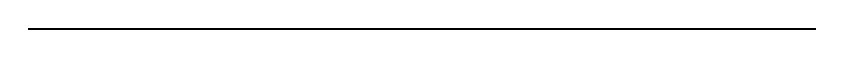
\begin{tikzpicture}
        \draw[fill=white] (-5.0, -0.01) rectangle (5.0, 0.01);
    \end{tikzpicture}
    \vspace{5px}

    \titlefont{PhD student}
}




% -- Mainbox de la segunda página

\posterbox[
    colback=white,
    valign=top,
    top=\inboxspacing,
    halign=left,
    left=\inboxspacing]
    {name=mainbox,
    below=headbox,
    column=1,
    span=1, % Toma el ancho completo de la página
    rowspan=\mainboxheight}
{
    \begin{tabular}{>{\footnotesize}rl}
    \centering

        2020
            & \textbf{Structure and electrocatalytic activity toward ORR of metallo-porphyrin networks} \\
            & J. M. Lombardi, D. Grumelli, Gutzler, K. Kern, H.F. Busnengo, P.N. Abufager \\
            & 2020 Express Conference on the Physics of materials and its application in Energy and enviroment \\
            & 3th August - 6th August \\
            & \smallspace

        2019
            & \textbf{Structure and catalytic activity of metalloporphyrin networks} \\
            & J. M. Lombardi, D. Grumelli, R.Gutzler, K. Kern, H. F. Busnengo and P. Abufager \\
            & Gordon Research Conference on Dynamics at Surfaces (GRC) \\
            & 28 de julio al 2 de Agosto, Newport, RI United States \\
            & \smallspace

        2019
            & \textbf{Structure and catalytic activity of metalloporphyrin networks} \\
            & J. M. Lombardi, D. Grumelli, R.Gutzler, K. Kern, H. F. Busnengo and P. Abufager \\
            & Gordon Research Seminar on Dynamics at Surfaces (GRS) \\
            & 27-28 de Julio, Newport, RI United States \\
            & \largespace

        2018
            & \textbf{On-surface transmetalation of metalloporphyrins self-assembled monolayers} \\
            & J. M. Lombardi, D. Hötger, P. Abufager, C. Morchutt, P. Alexa, D. Grumelli, J.Dreiser, S. Stepanow,\\
            & H. F. Busnengo, M. Etzkorn, R.Gutzler and K.Kern \\
            & VI San Luis Conference on Surfaces, Interfaces and Catalysis, Santa Fe (Argentina), June, 2018 \\
            & \smallspace
            
        & \titlefont{Contributions presented at Argentinian scientific} \\ 
        & \titlefont{and technological meetings} \\
        \hline \mediumspace

        & \textbf{Reacción de Reducción de Oxígeno en redes 2D de FePC/Au(111): efecto de moléculas} \\ 
        & \textbf{de solvente co-depositadas.} \\ 
        & J.M. Lombardi, H.F. Busnengo, P.Abufager, D.Grumelli \\
        & NANO 2022, Río Cuarto, 9-11 Agosto 2022 \\
        & \smallspace

        & \textbf{Propiedades catalíticas frente a la Reacción de Reducción de Oxígeno de estructuras} \\
        & \textbf{metal-orgánicas bidimensionales: porfirinas metálicas en Au(111)}\\ 
        & J.M. Lombardi, H.F. Busnengo, D.Grumelli, P.Abufager \\
        & NANO 2022, Río Cuarto, 9-11 August 2022 \\
        & \textcolor{hl0}{\textbf{Award for Best e-Poster Presentation}} \\
        & \smallspace

        & \textbf{Propiedades catalíticas frente a la Reacción de Reducción de Oxígeno de estructuras} \\
        & \textbf{metal-orgánicas bidimensionales: porfirinas metálicas en Au(111).} \\
        & J.M.Lombardi, H.F.Busnengo, D.Grumelli, P.Abufager. \\
        & IX Encuentro de Física y Química de Superficies y I Encuentro de Biología de Superficies, \\
        & 26-28 octubre 2022, Santiago del Estero. Semi-plenary Conference \\
        & \smallspace

        & \textbf{Estructura y actividad catalítica de redes de metaloporfirinas}\\
        & J. M. Lombardi, D. Grumelli, Gutzler, K. Kern, H.F. Busnengo, P.N. Abufager. \\
        & NANO 2019: XIX Encuentro de superficies y materiales \\
        & nanoestructurados, 5-7 June 2019, BsAs, Argentina \\
        & \smallspace

        & \textbf{Expositores XIII Jornada de Ciencia y Tecnología.}\\ 
        & Luque, E.; Frattini, A.; Oliveros, M.; Batista da Silva, M. Lombardi J. M. \\
        & (2019) \\
        & \smallspace

        & \textbf{Construcción de equipamiento de bajo costo para el Laboratorio de Física de la FCByF de la UNR.} \\
        & M.Oliveros, M.Batista de Silva, J.M.Lombardi, E.Luque, A.Frattini. \\
        & VI Jornadas de Física Aplicada a las Ciencias Biomédicas Rodolfo J. Rasia. 2019 \\
        & \smallspace

    \end{tabular}
    
}


% -- Footbox de la segunda página

\posterbox[colback=minimal-main]
    {name=footbox,
    below=mainbox,
    column=1,
    span=1,
    rowspan=\footboxheight}{}

\end{tcbposter}



























\begin{tcbposter}[
    poster = {columns=1, rows=1, spacing=0pt},
    boxes = {sharp corners, halign=center, valign=center, boxrule=0pt}
]

% -- Headbox
\posterbox[
    colback=minimal-main,
    halign=center]
    {name=headbox,
    span=1,
    rowspan=\headboxheight}
{
    \color{white}

    \header{Lombardi}{Juan}{Manuel}

    \vspace{-7px}
    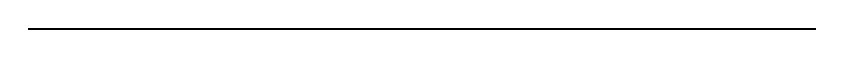
\begin{tikzpicture}
        \draw[fill=white] (-5.0, -0.01) rectangle (5.0, 0.01);
    \end{tikzpicture}
    \vspace{5px}

    \titlefont{PhD student}
}




% -- Mainbox de la segunda página

\posterbox[
    colback=white,
    valign=top,
    top=\inboxspacing,
    halign=left,
    left=\inboxspacing]
    {name=mainbox,
    below=headbox,
    column=1,
    span=1, % Toma el ancho completo de la página
    rowspan=\mainboxheight}
{
    \begin{tabular}{>{\footnotesize}rl}
    \centering
        & \textbf{Restauracion de la multilinealidad en datos cromatograficos median un algoritmo basado} \\ 
        & \textbf{en análisis funcional de datos.} \\
        & J.M.Lombardi, M.Alcaraza, M.Montemurrob,  S.A.Bortolato. \\
        & 10° congreso de química analítica, (2019) \\
        & \smallspace

        & \textbf{On-surface transmetalation of metalloporphyrins self-assembled monolayers.} \\
        & J.M.Lombardi, D.Hötger, P.Abufager, C.Morchutt, P.Alexa, D.Grumelli, J.Dreiser, S.Stepanow, \\
        & H.F.Busnengo, M.Etzkorn, R.Gutzler and K.Kern. \\
        & VI San Luis Conference on Surfaces, Interfaces and Catalysis, 2018, Santa Fe, Argentina \\
        & \smallspace

        & \textbf{Cascada de clasificadores para la deteccion y cuantificacion de parasitos en celulas} \\
        & \textbf{infectadas con T.cruzi.} \\
        & J.M. Lombardi. \\
        & Workshop on Scientific Programming Techniques, February 26th to March 9th, 2018, \\
        & Universidad nacional de Quilmes (UNL). \url{https://wtpc.github.io/} \\
        & \smallspace

        & \textbf{Desarrollo de un nuevo algoritmo basado en análisis funcional para restaurar la multilinealidad} \\
        & \textbf{en datos cromatográficos.}\\
        & J.M.Lombardi, S.Bortolato. \\
        & 9th Analytical Chemistry Congress, November 7th to 10th, 2017, Rio Cuarto\\
        & \smallspace

        & \textbf{FDA on chemometrics. VIII Workshop Wavelets and Information Theory.}\\
        & J. M. Lombardi, S.Bortolato. \\
        & 9th-11th August 2016, Universidad Nacional de la Plata(UNLP) \\
        & \largespace
               
        % Add the rest of the contributions here

        & \titlefont{Recent Awards} \\
        \hline \mediumspace


        2022
            & \textbf{Best Flash Poster selected by the Scientific Committee of NANO XX.} \\
            & \smallspace

        2021
            & \textbf{BIO Hackathon 2nd place} \\
            & Córdoba-Santa Fe, October 14th and 16th, 2021 \\
            & \smallspace

        2017
            & \textbf{Nasa Space Apps Challenge - Winner} \\            & Category: best data analysis \\

        & \largespace

        & \titlefont{Skills} \\
        \hline \mediumspace

        & \textbf{Programming Skills (Most Relevant):} \\
        & Python, Matlab, C, C++, Java, openGL, R, Fortran, Cuda \\
        & Data science, Machine learning, Data mining \\
        & \smallspace

        & \textbf{Libraries (Most Relevant):} \\
        & Numpy,  Pandas, Numba, openCV, openGL, modernGL, pyopenCl, TensorFlow, Theano, \\ 
        & Keras, Sklearn, AMP, ASE \\
        & \smallspace

        & \textbf{Tools (Most Relevant):} \\
        & Visual studio, Sublime, Linux, VIM, VMD, Látex, Git, Blender, Photoshop, Ilustrator, Microsoft office, \\
        & libre office, VASP, Gaussian, Hyperchem.\\


    \end{tabular}
    
}


% -- Footbox de la segunda página

\posterbox[colback=minimal-main]
    {name=footbox,
    below=mainbox,
    column=1,
    span=1,
    rowspan=\footboxheight}{}

\end{tcbposter}

\end{document}